%% V1.0
%% by Gabriel Garcia, gabrcg@gmail.com
%% This is a template for Udacity projects using IEEEtran.cls

%% Be Udacious!

\documentclass[10pt,journal,compsoc]{IEEEtran}

\usepackage[pdftex]{graphicx}
\usepackage{cite}
\usepackage{booktabs}
\usepackage{listings}
\lstset{basicstyle=\ttfamily,
  breaklines=true}
\usepackage{hyperref}
\hypersetup{
    colorlinks=true,
    linkcolor=blue,
    filecolor=magenta,
    urlcolor=cyan,
}
\hyphenation{op-tical net-works semi-conduc-tor}

\begin{document}

\title{Udacity RoboND: Robotic Inference Project}

\author{Dewar, M.P.}

\markboth{Inference project, Robotic Nanodegree, Udacity}%
{}
\IEEEtitleabstractindextext{%

\begin{abstract}
This project presents three deep neural network inference models, two of which are classification models, with the third as an attempt at an object detection model. The first data set consists of conveyor belt data supplied by the Udacity RoboND course moving various objects. The 2nd and 3rd datasets consist of user collected data from monitor cameras overseeing a welding workcell involving people and an industrial robot arm. Leveraging off of the Deep Learning GPU Training System (DIGITS) webapp these models can be quickly and easily tested over popular CNN architectures, as well as pretrained networks. Both classification and object detection networks were applied to this data, where bounding box image annotation was applied using the Labelbox platform (\href{https://www.labelbox.com/}{https://www.labelbox.com/}).
\end{abstract}

% Note that keywords are not normally used for peerreview papers.
\begin{IEEEkeywords}
Robot, IEEEtran, Udacity, \LaTeX, deep learning.
\end{IEEEkeywords}}


\maketitle
\IEEEdisplaynontitleabstractindextext
\IEEEpeerreviewmaketitle

\section{Introduction}
\label{sec:introduction}

\IEEEPARstart{I}{mage} inference has been a high standing benchmark of computer vision application which has recently seen exponential progress thanks to new deep convolutional neural network architectures. Object detection, recognition, and classification can now be performed through training image data with these deep learning models. Since the breakthrough Deep Neural Network (DNN) AlexNet in 2012, the ImageNet classification challenge (ILSVRC) has given rise to some famous single model architectures (i.e. GoogLeNet, ResNet, and Inception) consistently increasing validation accuracy year after year \cite{DBLP:journals/corr/CanzianiPC16}. Currently, an increasing demand is being put on applying these convolutional DNNs onto embedded systems for inference about the outside world. Whether the application deals with robotic latency, bandwith constraints, connectivity problems, or memory limitations finding a balance between inference time, and model accuracy is becoming increasingly important \cite{UdacityLesson7}.

This project will attempt to utilize some of these image recognition, and object detection networks leveraging NVIDIA's Deep Learning GPU Training System (DIGITS) workflow that allows the user to quickly define networks, and train several models in parallel to easily experiment and focus on the designing the network rather than programming and debugging \cite{NvidiaDN}. Evaluation of the models accuracy and inference time will be conducted to determine if each model is appropriate for the given inference application. The first dataset will be a presupplied dataset involving grocery store items moving along a conveyor.

The user provided dataset will involve taking video monitoring footage from a robotic workcell at the authors place of work involving humans, and an industrial robotic arm. In industrial manufacturing facilities, human workers are required to work alongside large robotic arms. Many safeguards are put into place in order to protect the safety of human workers from industrial robots, including various safety checks done by the robotic controller. These safety checks can include safety zones, where when a worker enters the zone the robot is prohibited from entering that zone. A more effective system would be to utilize inference of the robots surrounding in order to recognize if a human is present, and to detect and localize the human within the robots workspace in real time. With the human properly recognized by the robot, the robot can work in and around the human without the human impeding the progress of the robot, and the robot not being a hazard to the human. This dataset of the robotic workcell will be split into two separate datasets to test both image recognition, and to attempt object detection using the DIGITS workspace.

\section{Background / Formulation}
\label{sec:background}

Evaluating metrics of various ImageNet models, Figure. \ref{DNNMetric}, reveals some interesting insights as to what network to focus on for achieving a target inference time of 10ms, and an accuracy of 75\%. While ImageNet networks through the years have consistently increased in validation accuracy, compute power and network parameters have also increased, decreasing inference time and the applicability of these networks for embedded systems.

\begin{figure}[thpb]
  \centering
  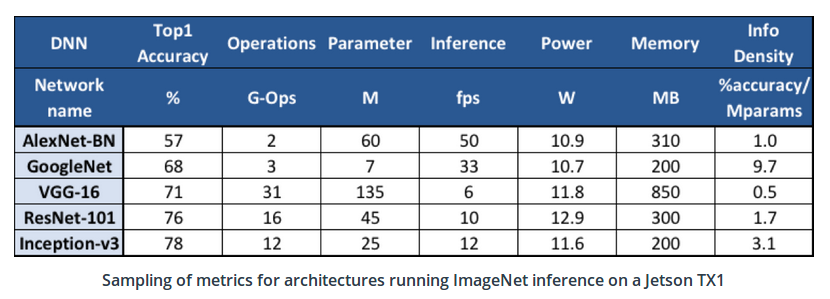
\includegraphics[width=\linewidth]{../img/DNN_metrics.png}
  \caption{Metrics of various DNN architectures show a hyperbolic relationship between inference time and accuracy.}
  \label{DNNMetric}
\end{figure}

GoogLeNet winner of ILSVRC 2014, focuses on a sparsely connected network architecture, increasing both network width and depth through the usage of inceptions blocks \cite{DBLP:journals/corr/SzegedyLJSRAEVR14}. This has major implications on reducing network parameters and memory/power usage, as well as maintaining a fairly fast inference time without drastic compromising accuracy. The use of inceptions blocks also helps combat overfitting to some extent. For all image recognition models in this project GoogLeNet will be used for the network architecture.

Based on the GoogLeNet fully-convolutional network (FCN), DetectNet take image data annotated with bounding boxes over areas of interest, and splits this image into a rectangular grid labelling areas of non-interest as "dontcare", and areas of interest with the pixel coordinates of the corners of the bounding box \cite{NvidiaDN}. A second data stream is also created as a coverage map of 0's and 1's indicating whether the object is present of not. Data is then fed through an augmentation phase to combat overfitting where the network will never be shown the same image twice, which is then fed into a sub-network GoogLeNet FCN without the data input layers, final pooling layer and output layers \cite{NvidiaDN}. Loss functions from the coverage maps, and bounding boxes are then grouped into a combined loss. Figure. \ref{detectNetStruct} shows the graphical structure of DetectNet.

\begin{figure}[thpb]
  \centering
  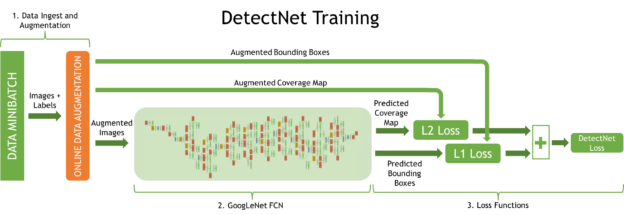
\includegraphics[width=\linewidth]{../img/detectnet_training.png} \\
  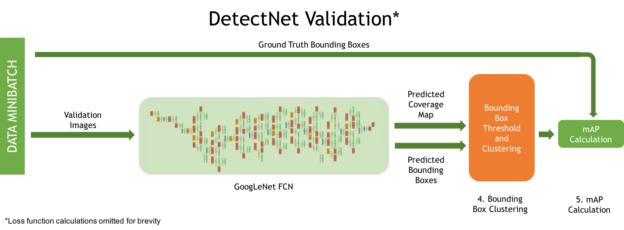
\includegraphics[width=\linewidth]{../img/detectnet_validation.png}
  \caption{DetectNet structure for training and vaidation respectively \cite{NvidiaDN}}
  \label{detectNetStruct}
\end{figure}

Measures graphed with tensorboard during model training of DetectNet of interest include \cite{NvidiaDN}:
\begin{itemize}
  \item \textbf{loss\_coverage}: the sum of squares of differences between the true and predicted object coverage
  \item \textbf{loss\_bbox}: the mean L1 loss (mean absolute difference) for the true and predicted corners of the bounding box for the object covered by each grid square.
  \item \textbf{mean Average Precision (mAP)}: score based on the product of the precision and recall for DetectNet. It is computed to measure model performance against the validation dataset.
\end{itemize}


\subsection{Conveyor Belt Data}

For the conveyor belt data classification images are to be classified as either a bottle, candy box, or nothing. Example images are provided in Figure. \ref{p1Data}, where these images are structured in the file format:

\begin{verbatim}
P1_data/
├── Bottle/
│   ├── Bottle_1.png
│   └── Bottle_2.png
├── Candy_box/
│   ├── Candy_box_1.png
│   └── Candy_box_2.png
└── Nothing/
  ├── Nothing_1.png
  └── Nothing_2.png
\end{verbatim}

\begin{figure}[thpb]
  \centering
  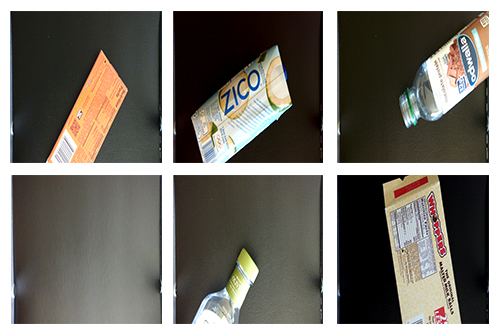
\includegraphics[width=\linewidth]{../img/P1-Dataset/dataset_sample.jpg}
  \caption{Sample dataset of Udacity supplied conveyor data}
  \label{p1Data}
\end{figure}

The model was trained over 10 epochs, using stochastic gradient decent (SGD), with a learning rate of 0.01 to prevent overfitting. Images were resized to 256x256 to reduce the compute power needed during training while still retaining sufficient resolution to extract the necessary features of the objects in order for the model to learn. Batch size was changed to 64, however the Telsa GPU used to train the data might have made this unnecessary.

\begin{figure}[thpb]
  \centering
  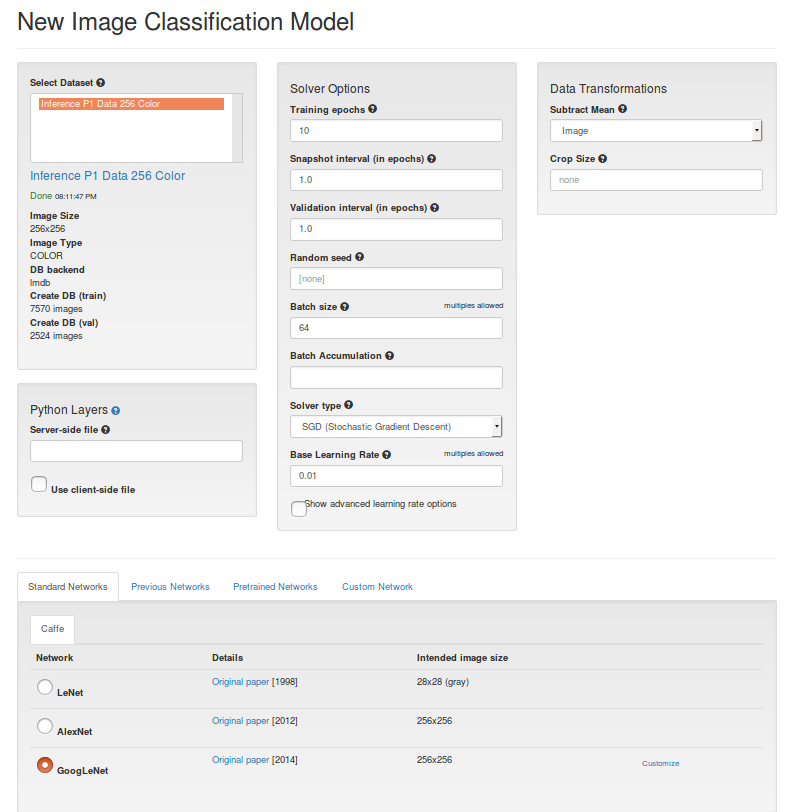
\includegraphics[width=\linewidth]{../img/P1-Dataset/P1-Model-Setup.png}
  \caption{DIGITS model setup for the conveyor belt dataset.}
  \label{p1ModelSetup}
\end{figure}


\subsection{Robot Workcell: Image Recognition}
\label{subsec:WC1Formulation}

For the first workcell images GoogLeNet was used again, this time training over 12 epochs for the first model. All hyperparameters were reused from the conveyor belt dataset resizing images to 256x256, at a learning rate of 0.01 using SGD.

An example of the training data is shown in Figure. \ref{workcell1Data} where the data is to be trained over four classes:

\begin{itemize}
  \item Person
  \item Robot
  \item Robot \& Person
  \item No one
\end{itemize}

\begin{figure}[thpb]
  \centering
  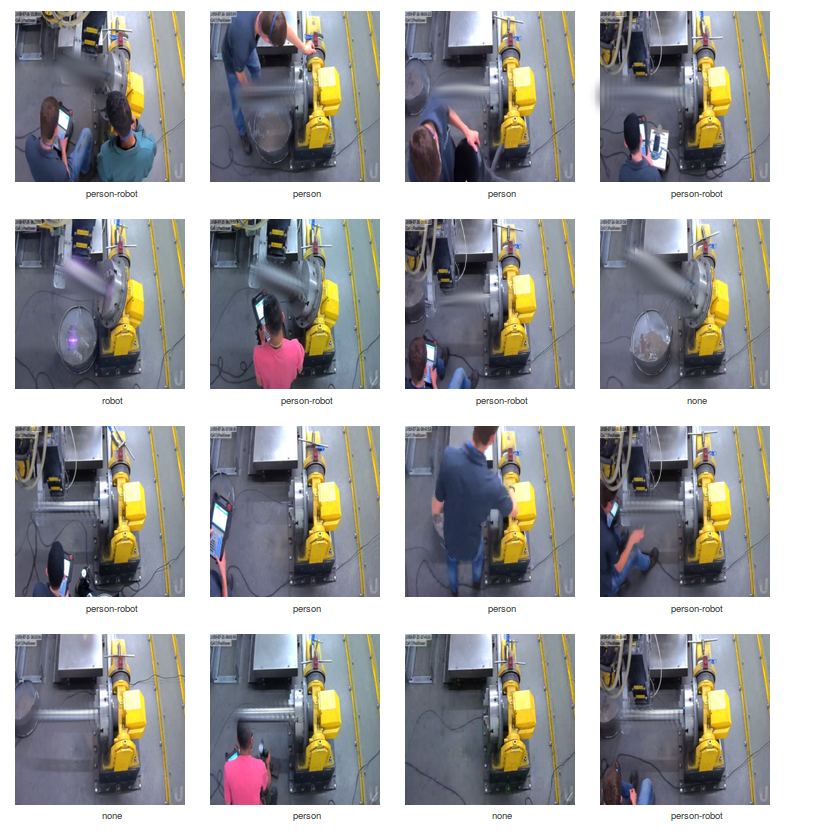
\includegraphics[width=\linewidth]{../img/Workcell1-Classification/dataset/WC1-labels.png}
  \caption{Sample dataset of the workcell1, where image classification should distinguish between whether there is just a robot in the image, just a person/people in the image, people and a robot in the image, or nothing in the image.}
  \label{workcell1Data}
\end{figure}

\subsection{Robot Workcell: Object Detection}

The next stage is to attempt object detection on the video feed to recognize where the robot and the workers are in the image. With the DIGITS object detection workspace the bounding box label data needs to be converted into the \href{http://www.cvlibs.net/datasets/kitti/}{KITTI} format. The KITTI format includes the 2D bounding box, 3d object dimensions, and 3d object location and rotation. The 3d object detection, and location metadata will be ignored in this project due to over complexity.

Images were padded by 100px, where padding is recommended by DIGITS, but images were not resized in an attempt to preserve spatial information (see Figure. \ref{workcell2Data}). Following the guide in NVIDIA's developer blog \cite{DNwDIGITS}, the Adaptive Moment Estimation (ADAM) solver was chosen as it may produce faster convergence for this type of network. learning rate was set to 1e-05, as anything greater than this number actually produced an error while running the model. Ref. \cite{DNwDIGITS} suggests selecting
'Exponential Decay' in the advanced learning options, but was ignored for the model used in this project. \href{https://github.com/dusty-nv/jetson-inference/blob/master/data/networks/detectnet.prototxt}{detectnet.prototxt} network was input into the custom network, pretrained with \href{http://dl.caffe.berkeleyvision.org/bvlc_googlenet.caffemodel}{bvlc\_googlenet.caffemodel} as it was strongly recommended to use pre-trained weights from an ImageNet-trained GoogLeNet \cite{DNwDIGITS} to decrease training times.

\begin{figure}[thpb]
  \centering
  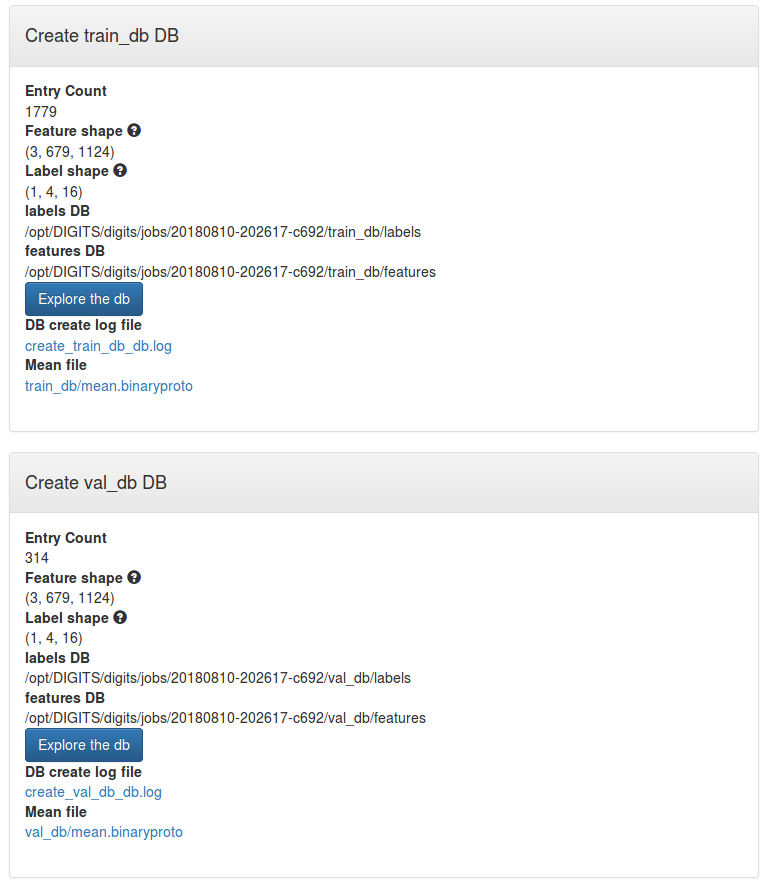
\includegraphics[width=\linewidth]{../img/Workcell2-Object-Detection/dataset/Workcell2-detectNet-Dataset3.png}
  \caption{Object detection dataset for workcell data}
  \label{workcell2Data}
\end{figure}

\begin{figure}[thpb]
  \centering
  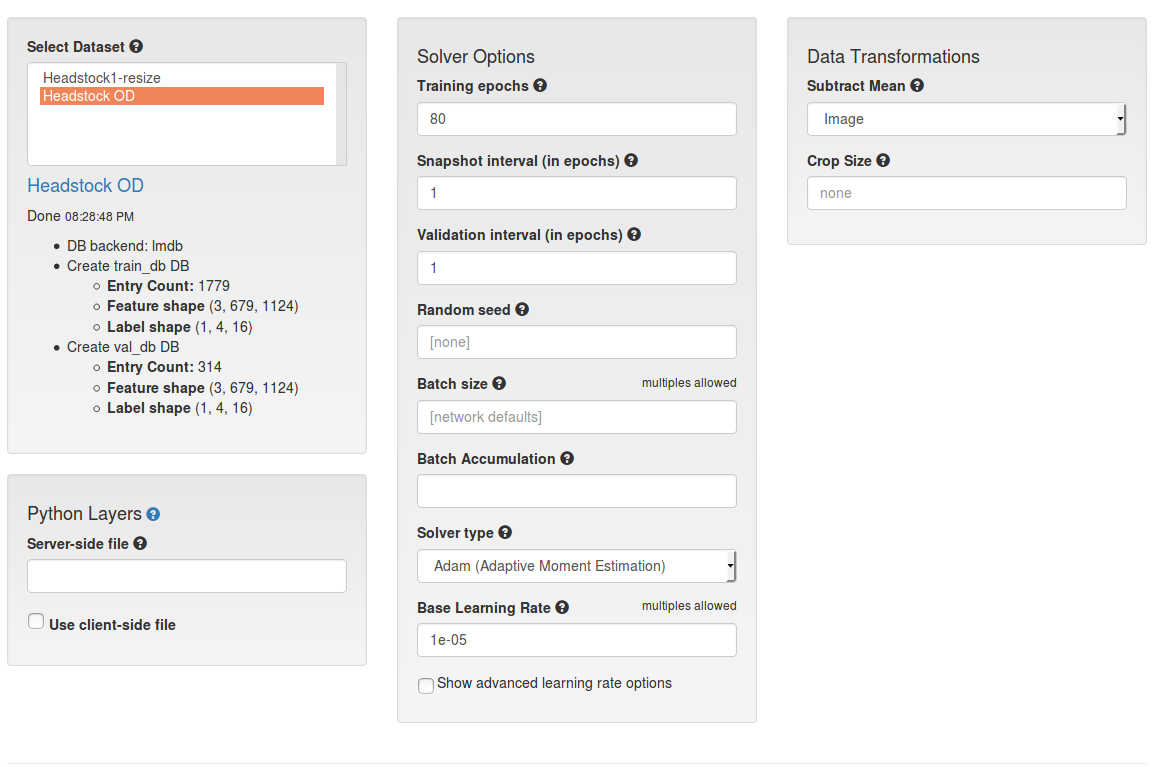
\includegraphics[width=\linewidth]{../img/Workcell2-Object-Detection/model/Workcell2-detectNet-Model01.png}
  \caption{DetectNet hyperparameters for workcell2 image data}
  \label{workcell2Model}
\end{figure}


\section{Data Acquisition}
\label{sec:dataAc}

Workcell image data was recorded from UniFi video cameras on the UniFi app randomly over the course of a week. These video feeds where downloaded, and screen captures where performed with VLC media player, and the images where sorted into a classification directory:

\begin{verbatim}
Workcell1/
├── Person/
│   ├── person00001.png
│   └── person00002.png
├── Person-Robot/
│   ├── person-robot00001.png
│   └── person-robot00002.png
└── Robot/
|    ├── robot00001.png
|    └── robot00002.png
└── None/
    ├── none00001.png
    └── none00002.png
\end{verbatim}

The sample size for the image data in workcell1 is broken down in Table. \ref{tab:WC1Data}. Image where kept in RGB Color and where 1024x579 px in size.
\begin{table}[h]
    \caption{Metadata for workcell 1 classification data}
    \begin{center}
    \begin{tabular}{lc}
    \toprule%
    Class & Sample Size\\\hline\noalign{\smallskip}
    Person & 552\\
    Person-Robot & 562\\
    Robot & 553\\
    None & 562\\\hline\noalign{\smallskip}
    Total & 2229\\
    \bottomrule%
    \end{tabular}
    \end{center}
    \label{tab:WC1Data}
\end{table}

The parent file was then uploaded to the Udacity VM to create the classification database for DIGITS. The DIGITS output after the dataset was created contained 1673 training images, and 556 validation images shown in Figure. \ref{workcell1DataInit}.

\begin{figure}[thpb]
  \centering
  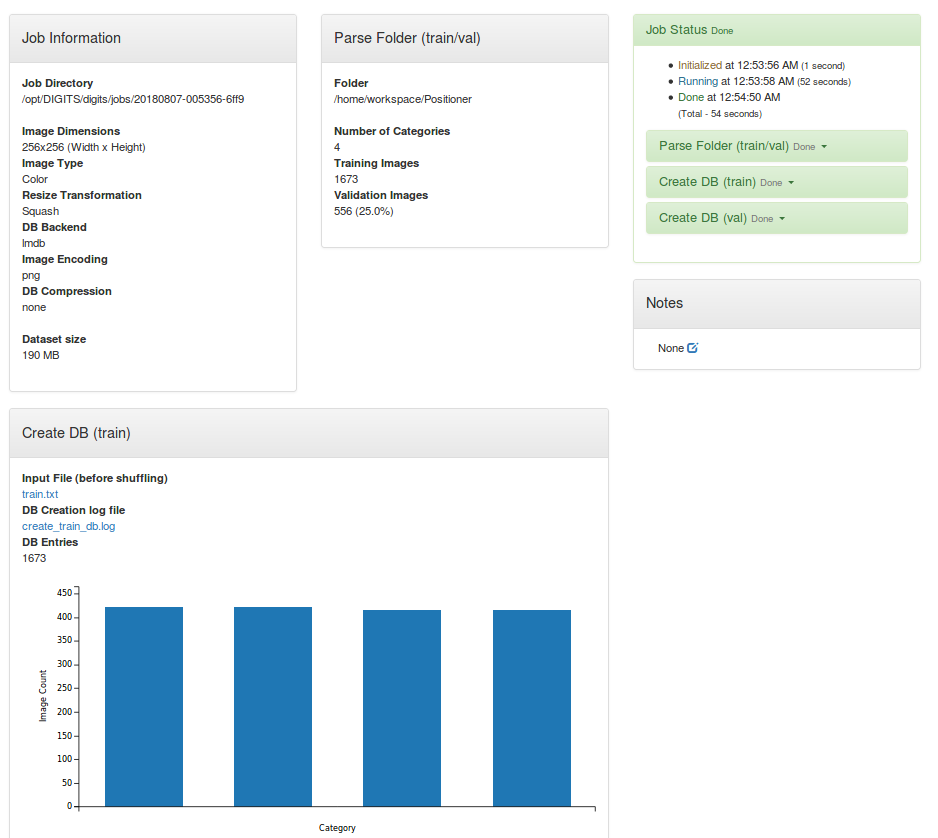
\includegraphics[width=\linewidth]{../img/Workcell1-Classification/dataset/WC1-dataset_initalization.png}
  \caption{DIGITS creation of workcell1 classification dataset}
  \label{workcell1DataInit}
\end{figure}

The object detection data for workcell2 was initially compiled the same way as workcell1. The image set was then uploaded to a Google Cloud storage bucket in order to be annotated by the \href{https://www.labelbox.com/}{labelbox} platform. Figure. \ref{labelboxAnnot} shows the labelling workspace used for drawing boxes around objects of interest, labelling them as either a person, or a robot, and classifying the image like that for workcell1.

\begin{figure}[thpb]
  \centering
  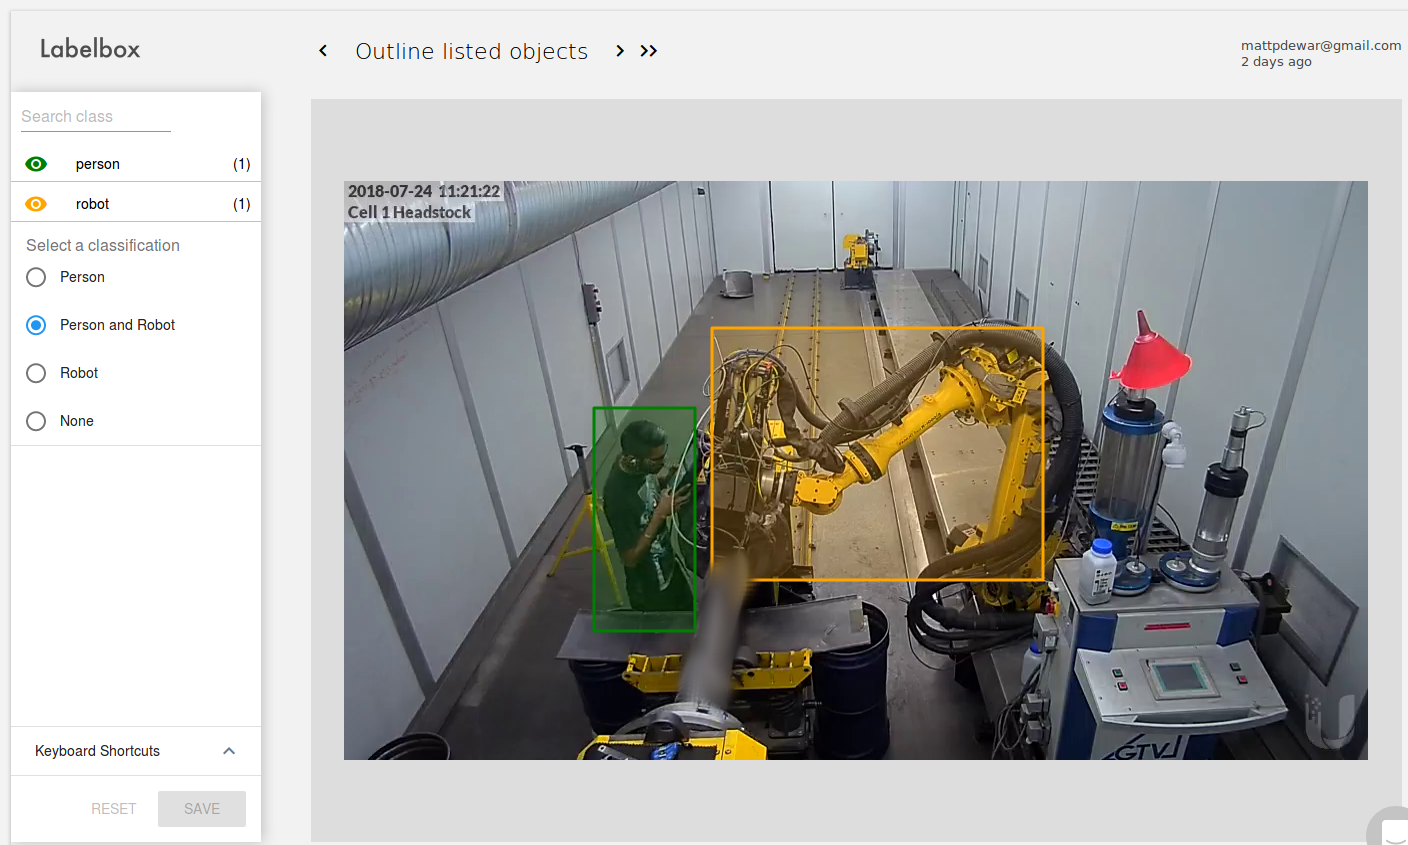
\includegraphics[width=\linewidth]{../img/Labelbox/labelbox-robot-person.png}
  \caption{Bounding box annotation using the Labelbox platform, where objects are recognized, and labelled as either a robot, or a person}
  \label{labelboxAnnot}
\end{figure}

The dimensions, and image type are the same as that of workcell1, where the sample sizes for each class can be found in Figure \ref{labelboxSamples}, where the total number of images is 2686.

\begin{figure}[thpb]
  \centering
  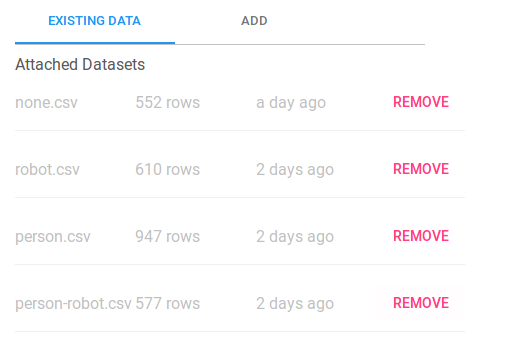
\includegraphics[width=\linewidth]{../img/Labelbox/labelbox_datasets.png}
  \caption{Sample Size for the workcell2 object detection dataset}
  \label{labelboxSamples}
\end{figure}

Exporting bounding box information from labelbox is in a Well Known Text (WKT) formatted JSON file. For DIGITS this data must be organized in the \href{https://devblogs.nvidia.com/deep-learning-object-detection-digits/}{KITTI} format with the file structure:
\begin{verbatim}
train/
├── images/
│   └── Robot00001.png
│   └── Person00001.png
│   └── Person-Robot00001.png
└── labels/
    └── Robot00001.txt
    └── Person00001.txt
    └── Person-Robot00001.txt
val/
├── images/
│   └── Robot00002.png
│   └── Person00002.png
│   └── Person-Robot00002.png
└── labels/
    └── Robot00002.txt
    └── Person00002.txt
    └── Person-Robot00002.txt
\end{verbatim}

Annotation information for each image is put into its own .txt file in the KITTI bounding box format, where the coordinate origin is located on the bottom left corner of the image:

\begin{lstlisting}
    robot 0 0 0 361.0 284.0 704.0 530.0 0 0 0 0 0 0 0 0
    person 0 0 0 194.0 34.0 322.0 315.0 0 0 0 0 0 0 0 0
\end{lstlisting}

In order to convert the WKT format from labelbox into the KITTI format we can utilize both the \href{https://github.com/Labelbox/Labelbox/tree/master/scripts}{Labelbox API} which can convert this JSON file into the COCO format, where then we can use the \href{https://github.com/dusty-nv/jetson-inference/blob/master/tools}{Jetson-Inference API}
along with the \href{https://github.com/cocodataset/cocoapi}{COCO API} to convert the COCO formatted labels into KITTI formatted labels. Detailed instructions on how to do this are located in the README.md file in the \textbf{./labelbox/} folder of this projects repository. It should be noted that when converting the WKT format to the KITTI format images with no objects had no associated label.txt file and therefore were not included in the dataset, lowering the total sample size to 2093 images.  From here the labels and images need to be sorted into the KITTI file format, separating them out into training and validation data. This was accomplished with a custom python script using sklearn to split the data. This script can be found in \textbf{./labelbox/scripts/kitti\_struct.py} of this directory. The produced data directory was then uploaded to the Udacity VM to be used with DIGITS, where the dataset metadata can be found in Figure. \ref{labelboxData}

\begin{figure}[thpb]
  \centering
  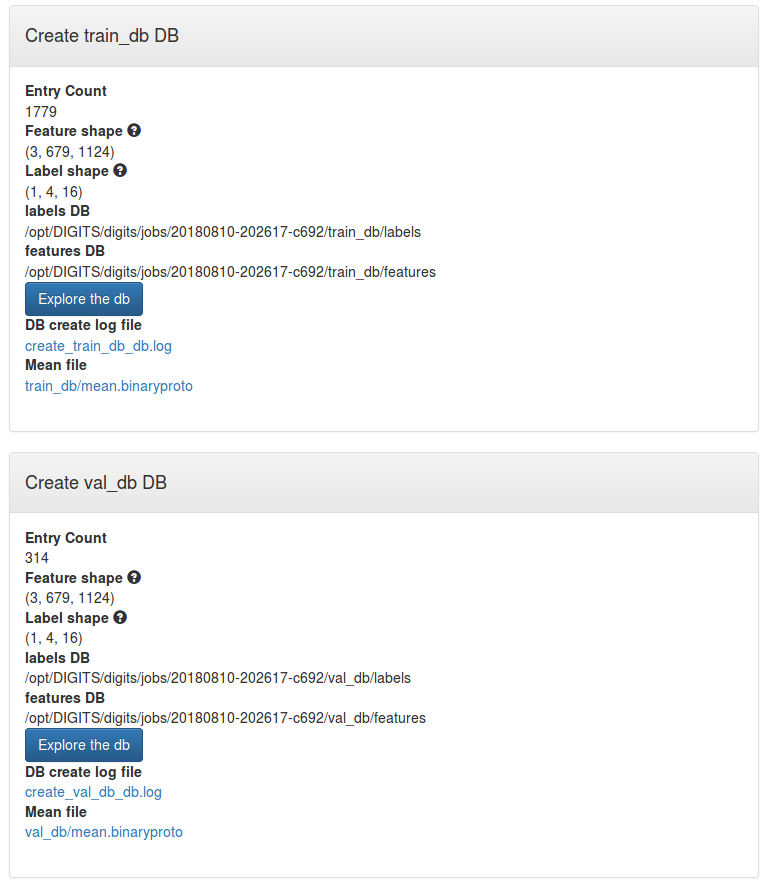
\includegraphics[width=\linewidth]{../img/Workcell2-Object-Detection/dataset/Workcell2-detectNet-Dataset3.png}
  \caption{Dataset for workcell2 object detection using DIGITS}
  \label{labelboxData}
\end{figure}

\section{Results}
\label{sec:results}

\subsection{Conveyor Belt Data}
The tensorboard of the model using the GoogLeNet Network in Figure. \ref{ConveyorTB} showing validation accuracies near 100\%. This is verified by running the model over the validation images in Figure. \ref{ConveyorVerification}. This model was saved in \textbf{ ./DIGITS/P1-Test\_Dataset/} of this repository. Running the evaluation command given by the project on an outside test dataset yielded a 75.4\% accuracy, and a $~5.3$ ms inference time, meeting the objectives of this project (see Figure. \ref{ConveyorEval}).

\begin{figure}[thpb]
  \centering
  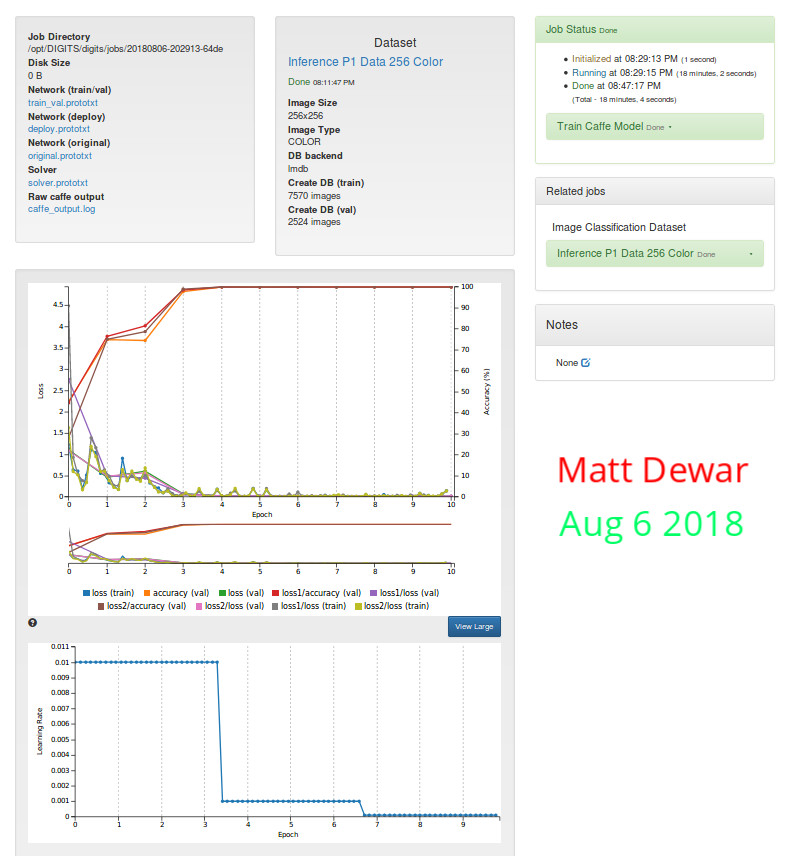
\includegraphics[width=\linewidth]{../img/P1-Dataset/P1-Model_GooGLeNet.jpg}
  \caption{Tensorboard Key indicators for the Conveyor belt model, where validation accuracy on the loss function is near 100\%, with the learning rate schedule for each epoch displayed on the bottom.}
  \label{ConveyorTB}
\end{figure}

\begin{figure}[thpb]
  \centering
  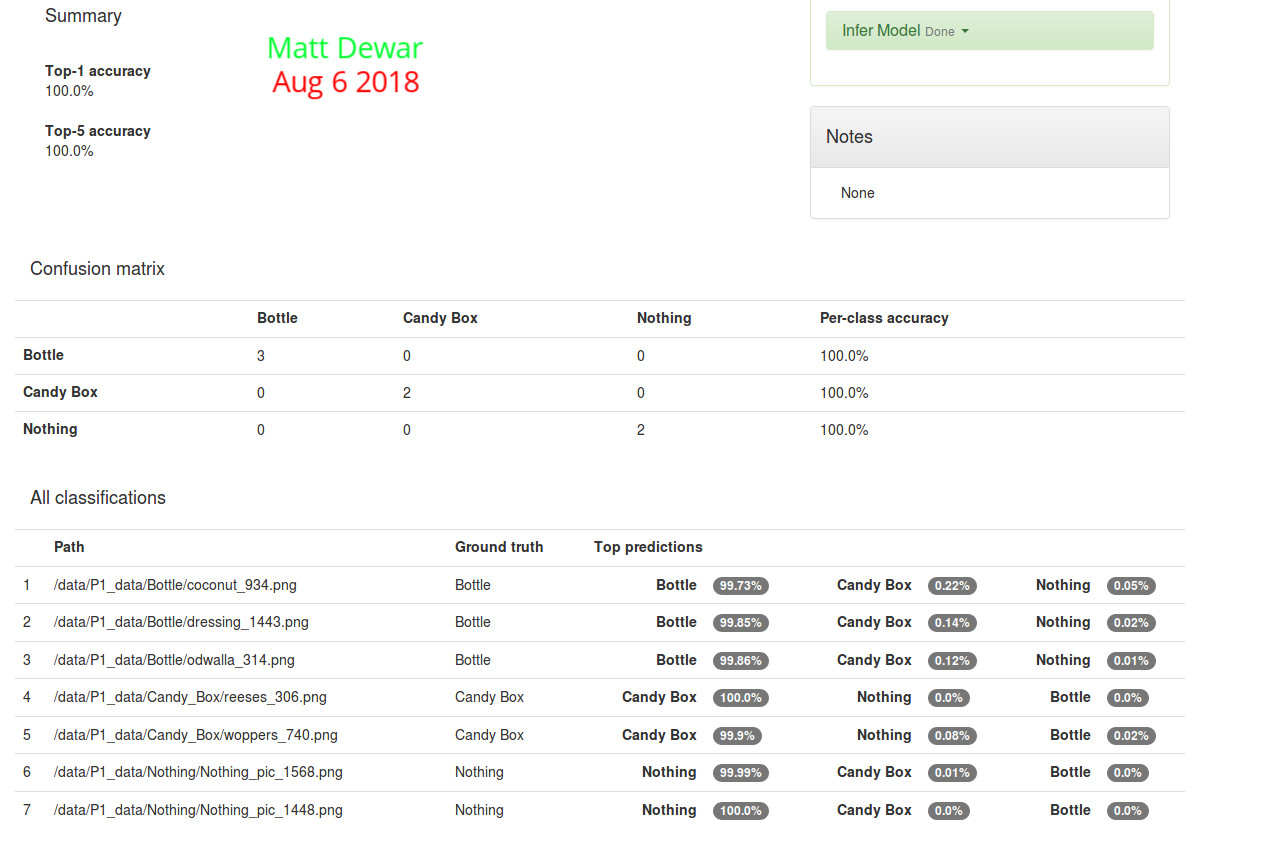
\includegraphics[width=\linewidth]{../img/P1-Dataset/P1-Prediction-Many.jpg}
  \caption{Conveyor model verification using the val.txt image files.}
  \label{ConveyorVerification}
\end{figure}

\begin{figure}[thpb]
  \centering
  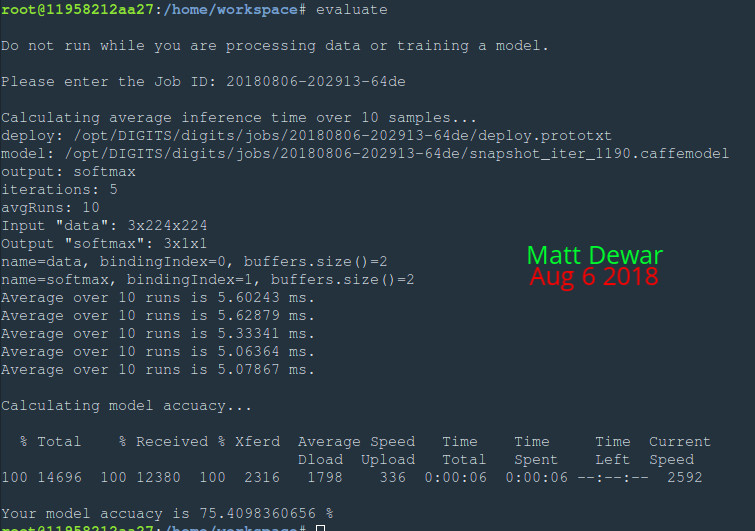
\includegraphics[width=\linewidth]{../img/P1-Dataset/P1-Model_GooGLeNet_evaluate.jpg}
  \caption{Conveyor model evaluation output}
  \label{ConveyorEval}
\end{figure}

\subsection{Robot Workcell: Image Recognition}

Training the workcell1 model using the same GoogLeNet network, and hyperparameters as in sub-section. \ref{subsec:WC1Formulation}, yielded a lower performance than with the conveyor belt dataset, where validation accuracies of the loss functions were just over 90\%, and an overall validation accuracy just above 80\%, seen in Figure. \ref{WC1-acc-loss}. Model verification in Figure. \ref{WC1-verification} shows some false positives when identifying people. This model can be found in \textbf{ ./DIGITS/Workcell1-Classification/GoogLeNet-initial/} for reference.

\begin{figure}[thpb]
  \centering
  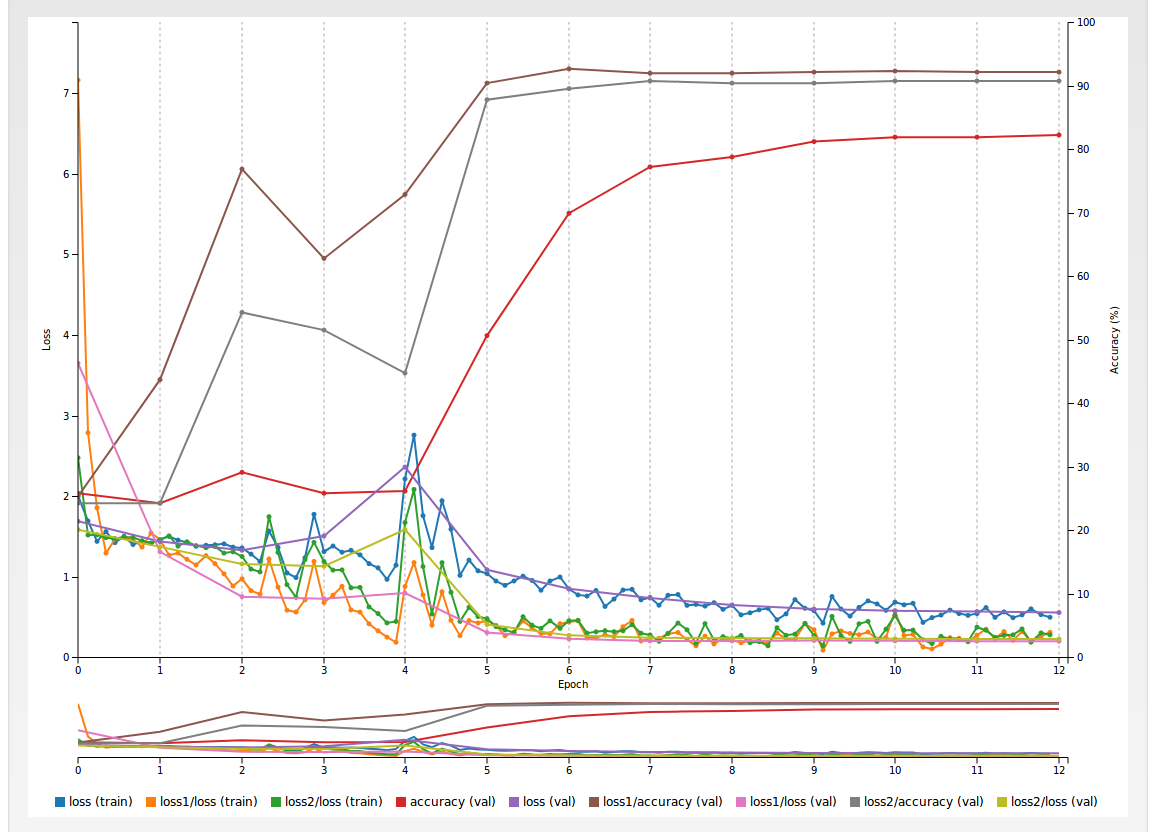
\includegraphics[width=\linewidth]{../img/Workcell1-Classification/initial/WC1-1-Loss-Accuracy.png} \\
  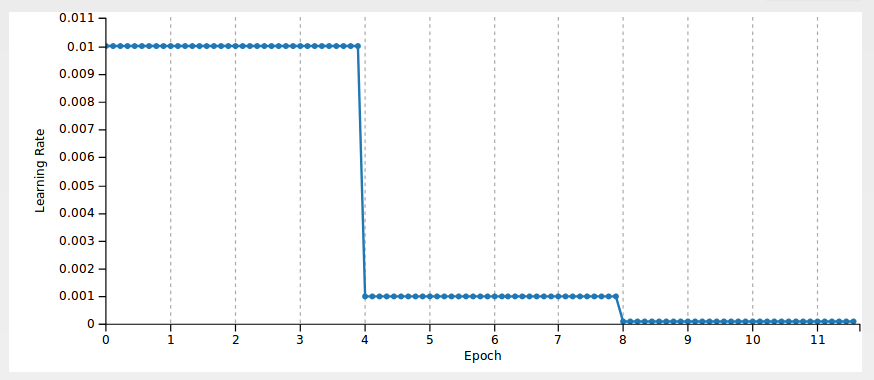
\includegraphics[width=\linewidth]{../img/Workcell1-Classification/initial/WC1-1-learning-rate.png}
  \caption{The top graph shows the network accuracy, and the bottom graph shows the learning rate schedule for the workcell1 recognition dataset.}
  \label{WC1-acc-loss}
\end{figure}

\begin{figure}[thpb]
  \centering
  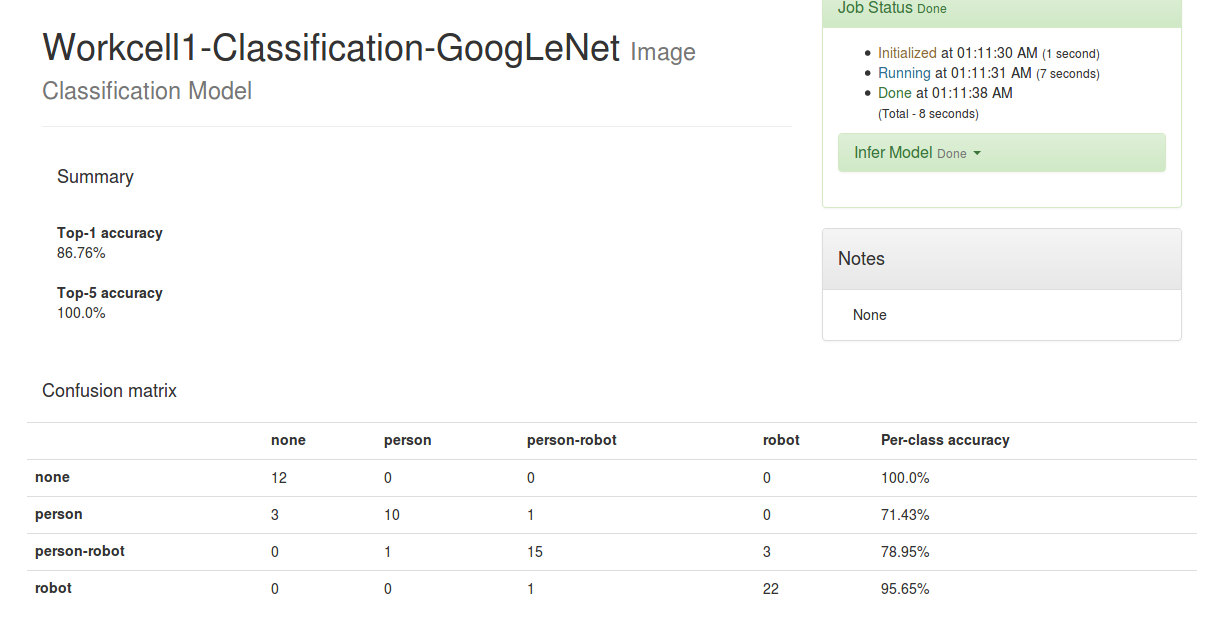
\includegraphics[width=\linewidth]{../img/Workcell1-Classification/initial/WC1-1-classification-test.png}
  \caption{Model verification of the workcell1 recognition dataset.}
  \label{WC1-verification}
\end{figure}

It was decided to train the model for another 12 epochs using the first model as a pretrained network. Results in Figure. \ref{WC1-acc-loss_2}, and Figure. \ref{WC1-verification_2} show a great improvement in validation accuracy, however a separate test dataset should be used to confirm the this model is nor subject to overfitting.  This model can be found in \textbf{ ./DIGITS/Workcell1-Classification/GoogLeNet-Run2/} of this projects repository.

\begin{figure}[thpb]
  \centering
  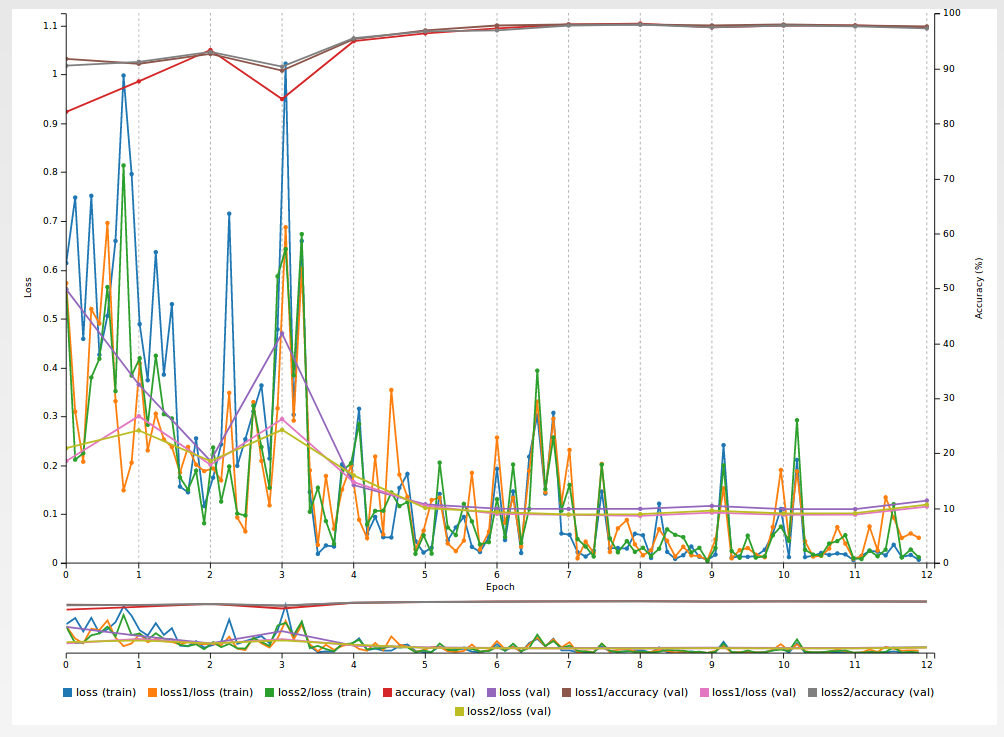
\includegraphics[width=\linewidth]{../img/Workcell1-Classification/Run2/WC1-2-Loss_accuracy.png} \\
  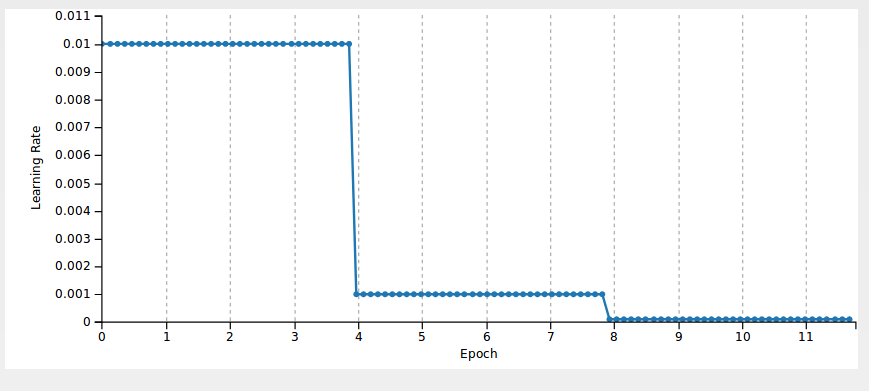
\includegraphics[width=\linewidth]{../img/Workcell1-Classification/Run2/WC1-2-LR.png}
  \caption{Training the workcell1 model for 12 more epochs improved the  validation accuracy to near near 100\%.}
  \label{WC1-acc-loss_2}
\end{figure}

\begin{figure}[thpb]
  \centering
  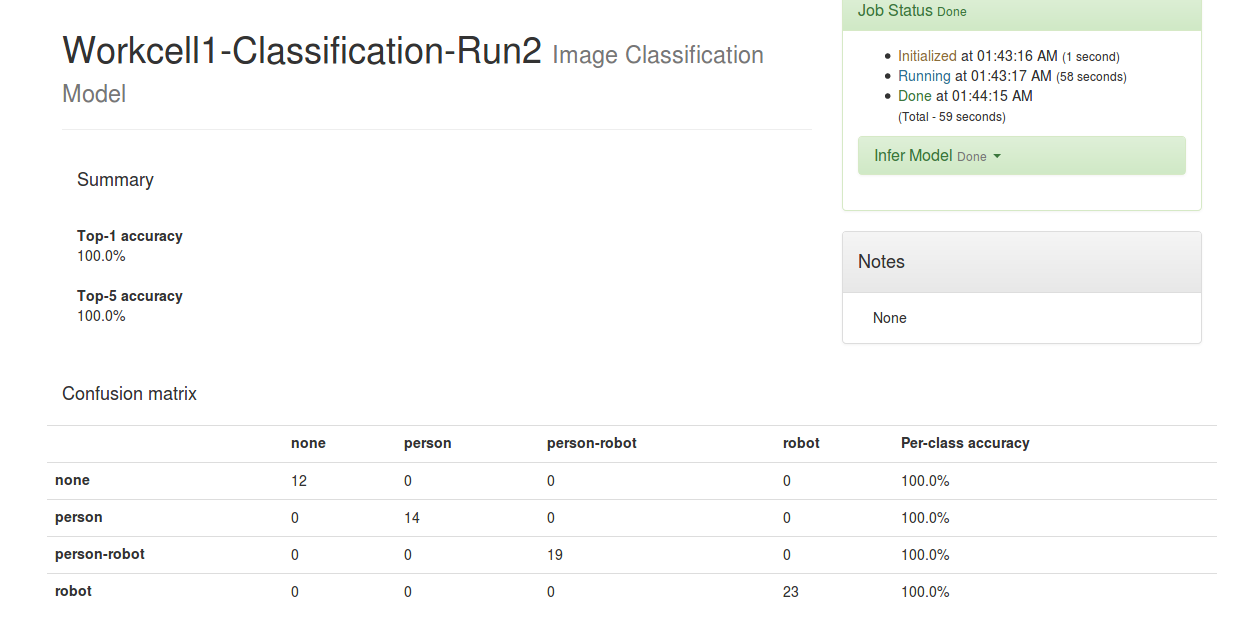
\includegraphics[width=\linewidth]{../img/Workcell1-Classification/Run2/WC1-2-Overfit.png}
  \caption{Model verification after training for 12 more epochs.}
  \label{WC1-verification_2}
\end{figure}


\subsection{Robot Workcell: Object Detection}

Setup for the object detection model can be found in Figure. \ref{WC2-model-setup}. The model was trained for 44 epochs with the tensorboard graphs of the training shown in Figure. \ref{WC2-acc-loss}. After 44 epochs the model does not seem to be improving with the loss coverage, and the loss bbox measures have not significantly improved during training and validation. mAP is generally used as the metric to determine the performance of the model. In Figure. \ref{WC2-acc-loss} it can be seen that the simplified mean Average Precision (mAP) score stay at 0\% after 44 epochs, where the model does not seem to be learning. This can be verified during model validation where no bounding boxes are found in any of the validation images (e.g. Figure. \ref{WC2-model-verif}). The DetectNet model can found in \textbf{ ./DIGITS/Workcell1-Object-Detection/Epoch-43}. Training this model for 44 epoch took a runtime of 4 hours on a Telsa GPU, therefore excessive experimentation to debug the model was not able to be done.

\begin{figure}[thpb]
  \centering
  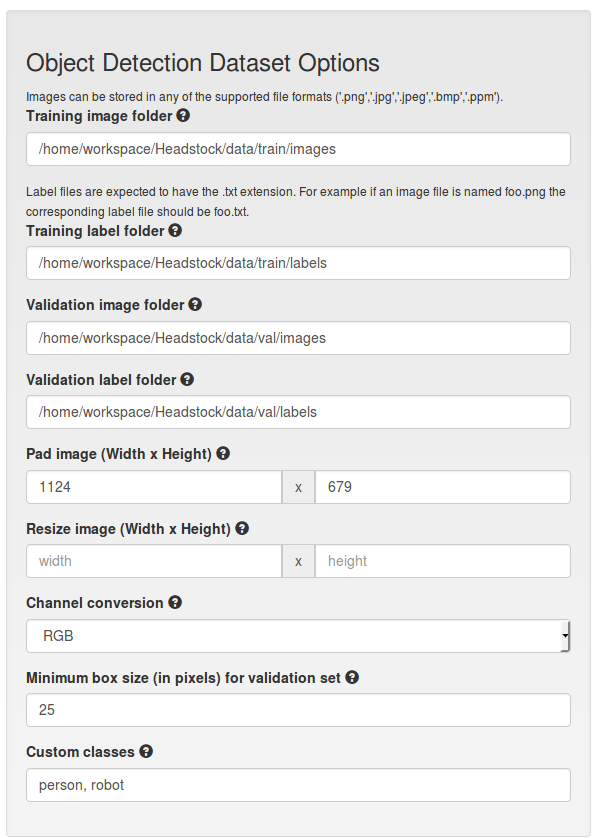
\includegraphics[width=\linewidth]{../img/Workcell2-Object-Detection/dataset/Workcell2-detectNet-Dataset.png}
  \caption{Model seetup for workcell2 object detection}
  \label{WC2-model-setup}
\end{figure}

\begin{figure}[thpb]
  \centering
  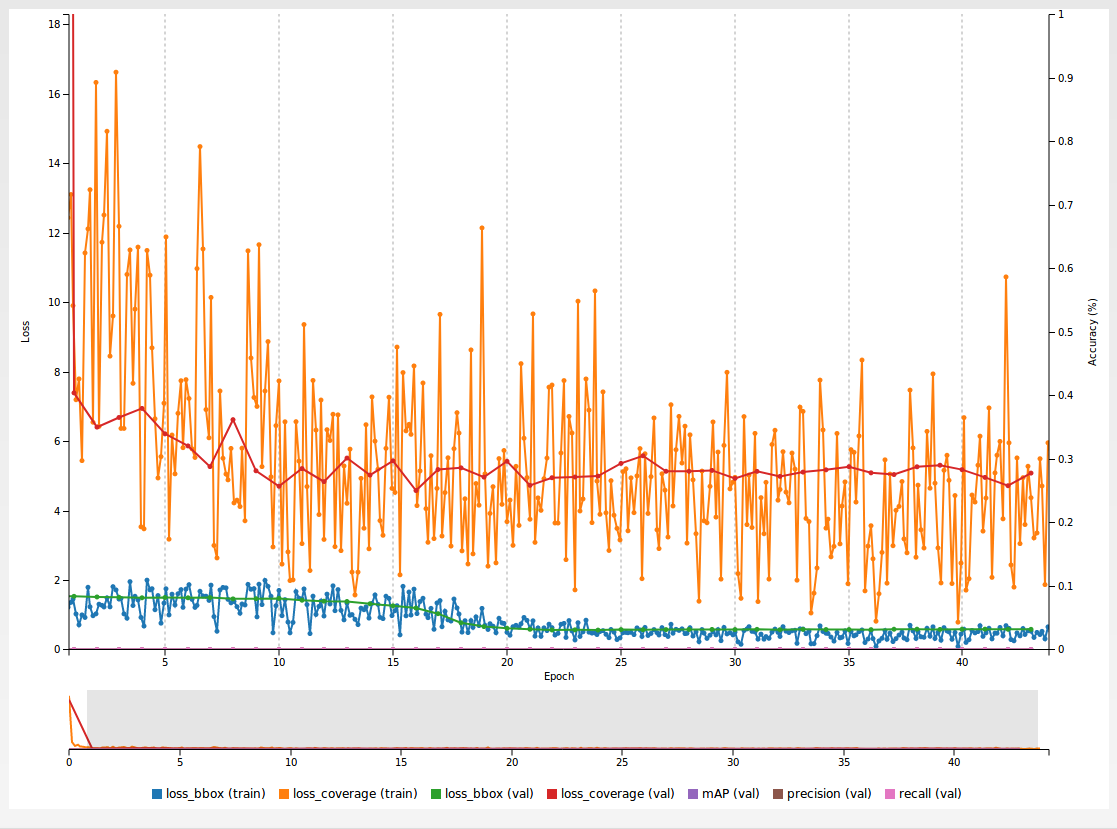
\includegraphics[width=\linewidth]{../img/Workcell2-Object-Detection/model/Workcell2-detectNet-Accuracy_loss.png} \\
  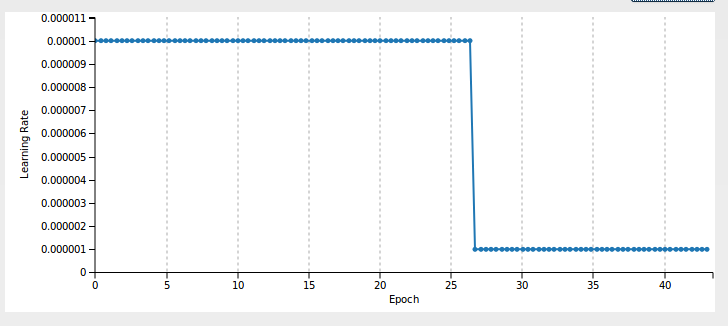
\includegraphics[width=\linewidth]{../img/Workcell2-Object-Detection/model/Workcell2-detectNet-LearningRate.png}
  \caption{Training of the workcell2 DetectNet model show after 44 epochs, the loss coverage, and loss bbox to not significantly decrease, and a mAP of essentially zero. Learning rate also fails to decay at an expected rate generally seen for object detection models.}
  \label{WC2-acc-loss}
\end{figure}

\begin{figure}[thpb]
  \centering
  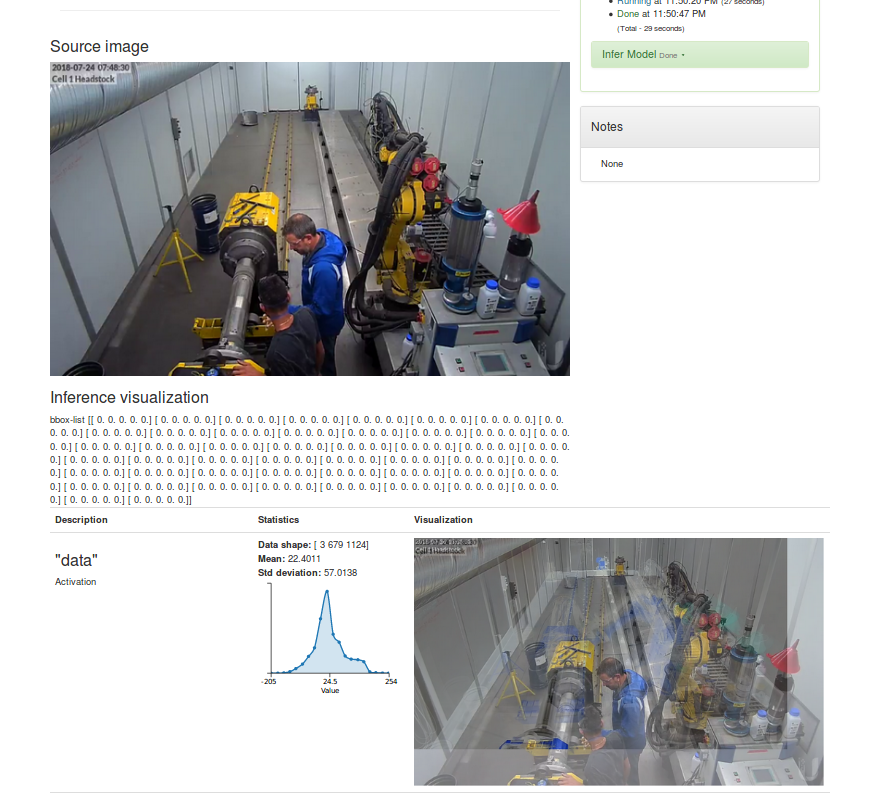
\includegraphics[width=\linewidth]{../img/Workcell2-Object-Detection/model/Workcell2-detectNet-ModelVerification01.png}
  \caption{Model verification for a single images shows that neither the people or the robot are recognized in the image.}
  \label{WC2-model-verif}
\end{figure}


\section{Discussion}
\label{sec:discussion}

The performance of the GoogLeNet model on the conveyor belt data show that this model is an excellent fit for this type of data. A decreased performance of this model on the robotic workcell dataset shows the increased complexity of this type of data compared to the conveyor data. Uncertainty with the results of the second model using the initial training as a pretrained network lies in the model verification showing 100\% per class in Figure. \ref{WC1-verification_2}. More test data should be accumulated for verification to decide if the model is potentially overfitted or not. If overfitting is occurring, the initial model should be retrained for more epochs instead of using a second model with a pretrained network.

The purpose of this project is firstly to provide a means for the robot controller to be able to detect when a person is in the workcell and if the mechanical arm is present within the same workspace. Secondly, the robot controller should be able to locate where that person is in the workcell as well as where the mechanical arm is, and if there is any potential conflict. The controller could then use this information to path plan around the person, or to stop or slow its motion to safely work around a detected person. Fast inference will be needed on the embedded platform/GPU on the deployed DNN in order for the robot controller to make quick and agile decisions. However high accuracy is much more important in limiting false-negatives that could lead to misjudgement, which would be a safety concern. Slower inference times can be handled as the robot will be limited in how quickly it can travel when a person can be present in the workcell.    

The failure of the DetectNet model to train can be thought to be from a number of factors. The KITTI formatted bounding box data was validated with a few pictures assuming that the origin is located at the bottom left of the image. This needs to be verified by looking at a jetson-inference object detection tutorial found at \href{https://github.com/dusty-nv/jetson-inference#locating-object-coordinates-using-detectnet}{https://github.com/dusty-nv/jetson-inference\#locating-object-coordinates-using-detectnet} using the \href{http://cocodataset.org/\#home}{MS-COCO} dataset. From doing the tutorial the author can gather greater inference on how the data needs to be formatted for a successful model. Ambiguity from the Labelbox platform in converting to the KITTI format, and running numerous API helper scripts in order to produce the correct file format may be causing mislabelled data, to where the network cannot be trained.

Another possible source of error was found in Ref. \cite{DNwDIGITS} where the learning rate can be seen to exponentially decay over epochs, where it was found that this is an option that can be selected under 'advanced learning rate options'. The padding and resizing option for the dataset should also be considered when looking for potential sources of error. Otherwise, training for more epochs should be attempted to see if a mAP score can be achieved after $>45$ epochs. If there are no errors in the current methodology then it can be concluded that the data is too complicated for given data size, and much more data will need to be attained in hopes of training the model.

\section{Conclusion/Future Work}
\label{sec:conclusion}

The conveyor belt product model show excellent results with the GoogLeNet Network obtaining a 75.4\% validation accuracy, and a $~5.3$ ms inference time.

The results of image recognition model look to be suitable to roll out for real time inference of the video monitor feed. The next step would be to see if the UniFi video can be streamed into the Jetson TX2 development board where the video feed can then be processed through the DetectNet model, and TensorRT. More data could always be used to improve the model, and to gather a test dataset for evaluation to test overfitting on the model.

The object detection network will need to be reworked as described in section \ref{sec:discussion} in order to see if this use case is suitable for the DetectNet network. If a successful model is generated than model evaluation should be done, and the video inference should be tested on on the jetson platform to see if the inference time is suitable for the produced model.


\bibliography{bib}
\bibliographystyle{ieeetr}

\end{document}
